\section{Drift: Intermediate Forms and Schedules}\label{sec:drift}

\subsection{Margins and routes}

Fix a space of shapes $\GG$ with a distance $d$, for instance the Euclidean distance between the control-point vectors of point-compatible outlines, or the distance between rendered bitmaps. A drifting edition presents at each position $p$ a letter $x$ in the shape $\rho_x(\alpha_x(p))$, and a reader can only use the presentation if distinct letters remain distinguishable throughout. Define the \emph{margin} of an edition as the smallest distance between the displayed shapes of two distinct letters over all positions at which both are in play,
\[
m \;=\; \min_{p}\ \min_{x\neq y}\ d\bigl(\rho_x(\alpha_x(p)),\,\rho_y(\alpha_y(p))\bigr).
\]
A legibility threshold $\theta>0$ is a property of readers and typefaces and is not derived here; the design requirement is simply $m\ge\theta$. The margin is determined by the routes $\rho_x$ and by the schedule $\boldsymbol\alpha$ jointly, and the results of this section show that the obvious choices of both can drive it to zero.

Between two fixed endpoints there are many routes. A glyph might change through the movement of its strokes, so that outlines deform continuously, through the successive replacement of its parts, so that a stem, a bowl or a terminal is exchanged for its counterpart in turn while the rest of the shape stays fixed, or through intermediate forms designed by hand specifically to preserve recognition, keyframes each of which is a good letter in its own right. These routes begin and end with identical alphabets and can differ greatly in what a reader experiences along the way. Neither the endpoints nor the schedule fixes the route, and the choice of route is a distinct design variable of the edition.

\subsection{Collision under linear exchange}

Let $a$ and $b$ be two letters whose destination shapes are exchanged, so that $\rho_a(0)=A$, $\rho_a(1)=B$, $\rho_b(0)=B$ and $\rho_b(1)=A$ for distinct shapes $A,B\in\GG$, where $\GG$ is a real vector space. Take the linear routes $\rho_a(\alpha)=(1-\alpha)A+\alpha B$ and $\rho_b(\alpha)=(1-\alpha)B+\alpha A$. Cross-dissolving two bitmaps is an example of such a route, because averaging images is linear interpolation in a vector space of images.

\begin{proposition}[Collapse of linear exchange]\label{prop:collapse}
Let $(\alpha_a,\alpha_b)$ be a schedule for the two letters that begins at $(0,0)$ and ends at $(1,1)$. (i) If the schedule is continuous, then at some position the letters $a$ and $b$ are displayed in the same shape. (ii) If the schedule takes only the values $0$ and $1$, each letter being either wholly original or wholly final, and changes one letter at a time, then the two letters are displayed in the same shape in the intermediate state.
\end{proposition}

\begin{proof}
The shapes coincide exactly when $\rho_a(\alpha_a)=\rho_b(\alpha_b)$, that is, when $(1-\alpha_a-\alpha_b)(A-B)=0$, and since $A\ne B$ this holds if and only if $\alpha_a+\alpha_b=1$. For (i), the function $f=\alpha_a+\alpha_b-1$ is continuous with $f=-1$ at the start and $f=+1$ at the end, so it vanishes somewhere by the intermediate value theorem. For (ii), the first change of one coordinate leaves the state at $(1,0)$ or $(0,1)$, where $\alpha_a+\alpha_b=1$; in the state $(1,0)$, for example, $a$ is already displayed in the shape $B$ and $b$ has not begun to move from $B$.
\end{proof}

A schedule that changes in discrete steps of intermediate size can step over the collision line without landing on it. It then avoids exact coincidence only by making an abrupt jump, and its distance from coincidence at the nearest sampled position is at most $|\alpha_a+\alpha_b-1|\,\|A-B\|$, which is small whenever the steps are fine. Exact collision is therefore the limiting case of a general near-collision, and the simultaneous jump of both letters from $(0,0)$ to $(1,1)$ is the only way to avoid it altogether, at the cost of the reader seeing the exchange all at once.

At the colliding position both letters share one glyph, which is the common point $(1-\alpha_a)A+\alpha_aB$, and in the synchronous case $\alpha_a=\alpha_b=\tfrac12$ it is the midpoint $\tfrac12(A+B)$. Figure~\ref{fig:morph} makes this visible for B and P by cross-dissolving rendered bitmaps. The first two rows show the stored letters B and P moving towards each other's shapes, and in the middle column the two rows are pixel for pixel identical, a fact verified by the program that drew the figure. A reader who sees this glyph cannot say from the shape alone which letter it stands for and must use context, which is exactly the loss of distinguishing information that the margin was defined to detect.

\begin{figure}[ht]
\centering
\begin{tikzpicture}
\node[anchor=south west,inner sep=0] (img) at (0,0) {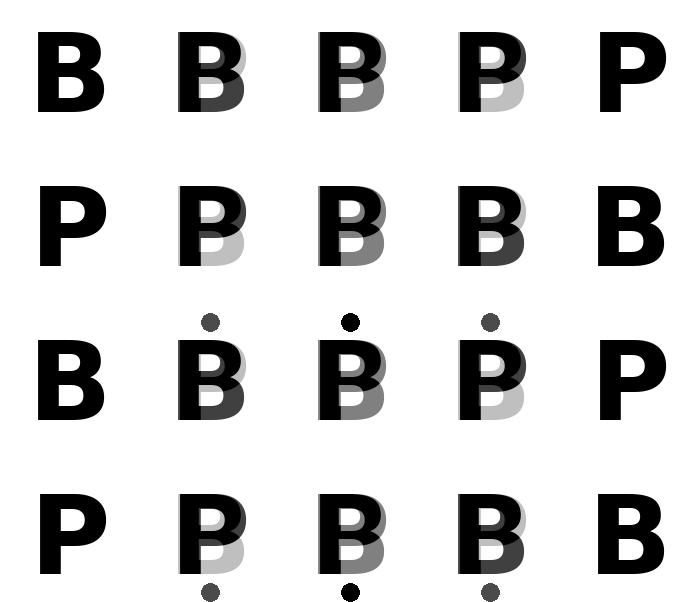
\includegraphics[width=0.78\textwidth]{out/morph.png}};
\begin{scope}[x={(img.south east)},y={(img.north west)}]
\foreach \i/\t in {0/0,1/0.25,2/0.5,3/0.75,4/1}{
  \node[font=\scriptsize,anchor=south] at ({(\i+0.5)/5},1.01) {$\alpha=\t$};}
\node[font=\scriptsize,anchor=east] at (-0.01,0.88) {B, linear};
\node[font=\scriptsize,anchor=east] at (-0.01,0.63) {P, linear};
\node[font=\scriptsize,anchor=east] at (-0.01,0.38) {B, detour};
\node[font=\scriptsize,anchor=east] at (-0.01,0.13) {P, detour};
\end{scope}
\end{tikzpicture}
\caption{Cross-dissolve of B and P rendered in DejaVu Sans Bold, with both letters at the same fraction $\alpha$ of the way to the other's shape. In the first two rows (linear routes) the two letters have identical glyphs at $\alpha=\tfrac12$. In the last two rows a mark above the stored B and below the stored P, with weight proportional to $\sin\pi\alpha$, keeps them distinct throughout and vanishes at both endpoints.}\label{fig:morph}
\end{figure}

The geometry can be drawn in the unit square of the pair of schedule values $(\alpha_a,\alpha_b)$. Every schedule is a path from the lower-left corner $(0,0)$ to the upper-right corner $(1,1)$, and the glyphs of the two letters coincide on the anti-diagonal $\alpha_a+\alpha_b=1$, which every such path must cross. Figure~\ref{fig:square} shows this, and also shows the two kinds of path discussed above: the synchronous path along the diagonal, which meets the anti-diagonal at the centre, and the one-letter-first path, which runs along the edges of the square and meets it at a corner.

\begin{figure}[ht]
\centering
\begin{tikzpicture}[scale=5.2,>=Stealth]
\draw[->] (0,0) -- (1.1,0) node[right]{$\alpha_a$};
\draw[->] (0,0) -- (0,1.1) node[above]{$\alpha_b$};
\draw (1,0.015) -- (1,-0.015) node[below]{\small 1};
\draw (0.015,1) -- (-0.015,1) node[left]{\small 1};
\draw[thick,red!70!black] (1,0) -- (0,1);
\draw[thick,blue!60!black] (0,0) -- (1,1);
\fill[blue!60!black] (0.5,0.5) circle (0.014);
\draw[thick,dashed,green!40!black] (0,0) -- (1,0) -- (1,1);
\fill[green!40!black] (1,0) circle (0.014);
\draw[thick,orange!80!black] plot[smooth] coordinates {(0,0) (0.15,0.3) (0.4,0.38) (0.5,0.7) (0.8,0.8) (1,1)};
% legend
\draw[thick,red!70!black] (1.3,0.92) -- (1.42,0.92) node[right,black,font=\small]{collision line $\alpha_a+\alpha_b=1$};
\draw[thick,blue!60!black] (1.3,0.80) -- (1.42,0.80) node[right,black,font=\small]{synchronous schedule};
\draw[thick,dashed,green!40!black] (1.3,0.68) -- (1.42,0.68) node[right,black,font=\small]{one letter first};
\draw[thick,orange!80!black] (1.3,0.56) -- (1.42,0.56) node[right,black,font=\small]{general schedule};
\end{tikzpicture}
\caption{Schedules of two exchanged letters as paths in the unit square. Under linear routes the displayed shapes coincide on the collision line, which every path from $(0,0)$ to $(1,1)$ meets.}\label{fig:square}
\end{figure}

\subsection{The detour}

The collision is a consequence of confining both routes to the straight line through $A$ and $B$. In a shape space of dimension at least two there is room to go around. Let $u\in\GG$ be a vector orthogonal to $A-B$ and $\lambda>0$, and replace the linear routes by
\[
\rho_a(\alpha)=(1-\alpha)A+\alpha B+\lambda\sin(\pi\alpha)\,u,\qquad
\rho_b(\alpha)=(1-\alpha)B+\alpha A-\lambda\sin(\pi\alpha)\,u .
\]
Both routes still begin and end at the original shapes, because $\sin(\pi\alpha)$ vanishes at $\alpha=0$ and $\alpha=1$, and in between the two letters pass on opposite sides of the line through $A$ and $B$.

\begin{proposition}[Detour]\label{prop:detour}
For the routes above, and for any schedule values $(\alpha_a,\alpha_b)\in[0,1]^2$, the displayed shapes of $a$ and $b$ coincide if and only if $(\alpha_a,\alpha_b)\in\{(1,0),(0,1)\}$. Along the synchronous path $\alpha_a=\alpha_b=\alpha$ the distance between the two shapes is
\[
\sqrt{(1-2\alpha)^2\|A-B\|^2+4\lambda^2\sin^2(\pi\alpha)\|u\|^2},
\]
which equals $\|A-B\|$ at the endpoints and, for $\mu=\lambda\|u\|/\|A-B\|<1/\pi$, attains its minimum $2\mu\,\|A-B\|$ at $\alpha=\tfrac12$.
\end{proposition}

\begin{proof}
The difference of the two shapes is $d=(1-\alpha_a-\alpha_b)(A-B)+\lambda\bigl(\sin\pi\alpha_a+\sin\pi\alpha_b\bigr)u$. Since $u\perp A-B$, $\|d\|^2=(1-\alpha_a-\alpha_b)^2\|A-B\|^2+\lambda^2(\sin\pi\alpha_a+\sin\pi\alpha_b)^2\|u\|^2$, and this is zero if and only if $\alpha_a+\alpha_b=1$ and $\sin\pi\alpha_a+\sin\pi\alpha_b=0$. On $[0,1]$ the sine is nonnegative, so the second condition forces $\sin\pi\alpha_a=\sin\pi\alpha_b=0$, hence $\alpha_a,\alpha_b\in\{0,1\}$, and together with the first condition this gives the two corners. The synchronous formula follows by substitution. Writing $\alpha=\tfrac12+\delta$ with $|\delta|\le\tfrac12$, the squared distance divided by $\|A-B\|^2$ is $4\delta^2+4\mu^2\cos^2(\pi\delta)$, and subtracting its value $4\mu^2$ at $\delta=0$ leaves $4\delta^2-4\mu^2\sin^2(\pi\delta)=4(|\delta|-\mu\sin\pi|\delta|)(|\delta|+\mu\sin\pi|\delta|)$. Because $\sin\pi|\delta|\le\pi|\delta|$ and $\mu\pi<1$, the first factor is positive for $\delta\ne0$, so the minimum is attained uniquely at $\delta=0$.
\end{proof}

Figure~\ref{fig:sep} plots the synchronous separation for three values of $\mu$. With $\mu=0$ the separation falls to zero at the midpoint, which is the collision, and with positive $\mu$ it keeps a floor of $2\mu\|A-B\|$. The result has one caution of its own, visible in the corner case: a detour does not protect a schedule that carries one letter all the way to its destination while the other has not yet begun, because the extra term vanishes at both endpoints, so the state $(0,1)$ shows $b$ in the original shape of $a$. The schedule must therefore keep the pair away from the opposite corners, and in practice this means moving the two letters of a pair together or interleaving their steps closely.

\begin{figure}[ht]
\centering
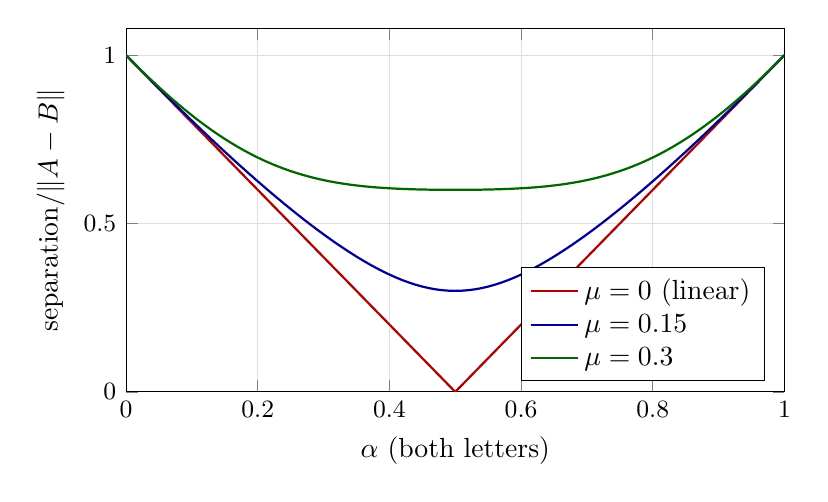
\begin{tikzpicture}
\begin{axis}[width=0.82\textwidth,height=6.2cm,xlabel={$\alpha$ (both letters)},ylabel={separation$/\|A-B\|$},
  xmin=0,xmax=1,ymin=0,ymax=1.08,legend pos=south east,legend cell align=left,
  grid=both,grid style={gray!25},tick label style={font=\small}]
\addplot[domain=0:1,samples=101,thick,red!70!black]{sqrt((1-2*x)^2+4*0*sin(deg(pi*x))^2)};
\addlegendentry{$\mu=0$ (linear)}
\addplot[domain=0:1,samples=101,thick,blue!60!black]{sqrt((1-2*x)^2+4*0.15^2*sin(deg(pi*x))^2)};
\addlegendentry{$\mu=0.15$}
\addplot[domain=0:1,samples=101,thick,green!40!black]{sqrt((1-2*x)^2+4*0.3^2*sin(deg(pi*x))^2)};
\addlegendentry{$\mu=0.3$}
\end{axis}
\end{tikzpicture}
\caption{Distance between the displayed shapes of two exchanged letters under the detour routes of Proposition~\ref{prop:detour}, as a fraction of the distance between the endpoint shapes. The parameter $\mu$ is a geometric parameter of the model and has no empirical status.}\label{fig:sep}
\end{figure}

The detour has a historical analogue in the Arabic script. Many Arabic letters share a skeleton and are distinguished by the number and position of dots, a system in which the skeletal forms of early texts were supplemented by dotting to separate letters that the skeleton alone left ambiguous \citep{daniels1996}. A mark that is orthogonal to the dimension along which two letters are confusable is exactly what the detour supplies. The last two rows of Figure~\ref{fig:morph} realise it with a dot placed above one letter and below the other, with weight proportional to $\sin\pi\alpha$. Whether such marks help or hinder reading, and whether they leave residue that interferes with the final forms, are empirical questions, and the proposition says only that the geometric obstacle can be removed at the cost of intermediate glyphs that are not letters of either endpoint alphabet.

\subsection{Longer cycles}

The collision of Proposition~\ref{prop:collapse} is specific to exchange of two letters. Take a three-cycle $a\to b\to c\to a$ with distinct shapes $A,B,C$, so that $a$ moves from $A$ to $B$, $b$ from $B$ to $C$, and $c$ from $C$ to $A$, each along a linear route with a common parameter $\alpha$.

\begin{proposition}[Three-cycles]\label{prop:cycles}
If $A,B,C$ are affinely independent, no two of the three letters are displayed in the same shape for any $\alpha\in[0,1]$.
\end{proposition}

\begin{proof}
The shapes at parameter $\alpha$ are $(1-\alpha)A+\alpha B$, $(1-\alpha)B+\alpha C$ and $(1-\alpha)C+\alpha A$. The difference of the first two is $(1-\alpha)A+(2\alpha-1)B-\alpha C$, a combination of $A,B,C$ whose coefficients sum to zero. By affine independence such a combination vanishes only if all coefficients vanish, but $1-\alpha=0$ forces $\alpha=1$ and then $2\alpha-1=1\ne0$. The other two differences are obtained by cyclic relabelling.
\end{proof}

Affine independence holds for any three points not on a common line, so it is the generic case in a shape space of any realistic dimension. The consequence for design is a trade-off. Reciprocal alphabets are self-inverse and simple to document but cannot be drifted by a shared linear parameter without collision, whereas three-cycles can, at the cost of distinct tables for encoding and decoding. The alternative for reciprocal alphabets is the detour of the preceding subsection. A further remark concerns topology. The space of ordered pairs of distinct points in $\mathbb{R}^n$ is homotopy equivalent to the sphere $S^{n-1}$, so for $n=2$ there are inequivalent ways of exchanging two points, clockwise and anticlockwise, while for $n\ge3$ every route is topologically equivalent to every other. In a high-dimensional shape space, therefore, routes between the same endpoints are not distinguished by their topology, and the differences that matter between them are quantitative: the margin, the legibility of the intermediate forms, and the exposure they allow.

\subsection{Cycles of presentation}

Nothing in the formalism requires the schedule to be monotone or the endpoint to be final. A route can pass through a hybrid script on the way from Latin to Standard Galactic and continue back to Latin, so that forms learned in the middle of the book return in the context of the original alphabet. Formally this is a route whose parameter is a loop in $\GG$, with the source shape of each letter also its last. Such a design changes the empirical question in an interesting way. A reader who recovers the original form after passing through the hybrid has had the opportunity to learn the association between the two while reading, and a test after the return can ask whether the intermediate forms are still recognised, which is a measure of retention independent of the final state. It also doubles the number of occasions on which the schedule must avoid collisions, since the same pairs of letters are crossing in both directions, and the discussion of exposure below applies to each leg.

\subsection{Exposure and the novelty load}

A schedule changes shapes as a function of position, but what a reader learns depends on the number of occasions on which each shape is seen, and these are tied to position through the frequency of letters. Let $p_\ell$ be the relative frequency of letter $\ell$ in the text and $N_\ell(p)$ the number of occurrences of $\ell$ before position $p$. A schedule that is uniform in position gives every letter the same fraction of the transition at the same point of the book and therefore gives it exposures in proportion to frequency, whereas a schedule that is driven by exposure advances each letter after a fixed number of its own occurrences, for instance
\[
\alpha_\ell(p)=\min\Bigl(1,\max\bigl(0,\tfrac{N_\ell(p)-D_\ell}{KS}\bigr)\Bigr),
\]
where $D_\ell$ is a delay in occurrences before the letter begins to change, $S$ is a number of stages, and $K$ is the number of exposures required per stage.

To see what position-uniform schedules imply, take a model book of 80{,}000 words with 4.7 letters per word on average, a modelling assumption rather than a measurement, giving $L=376{,}000$ letters, and take standard English letter frequencies \citep{lewand2000}. Divide the book into $S=5$ equal stages of 75{,}200 letters. The letter E, with relative frequency 12.7 per cent, is seen about 9{,}550 times in each stage, and Z, with 0.074 per cent, about 56 times, a ratio of 172 to 1, which is the ratio of the frequencies. Table~\ref{tab:exposure} gives the figures for a selection of letters, together with the length of text a letter needs to reach its final form under an exposure-driven schedule with $K=40$ and $S=5$, that is, 200 exposures in all. The most frequent letters complete in a few hundred words, while Z needs about 270{,}000 letters, 72 per cent of the model book, and this means that it spends most of the book in transition. The numbers $K=40$ and $S=5$ are illustrative values with no empirical standing.

\begin{table}[ht]
\centering
\small
\begin{tabular}{crrrr}
\toprule
Letter & Freq. & Per stage, uniform & To final stage, exposure-driven & In words\\
\midrule
e & 12.70\% & 9\,552 & 1\,575 & 335\\
t & 9.06\% & 6\,810 & 2\,208 & 470\\
a & 8.17\% & 6\,142 & 2\,449 & 521\\
n & 6.75\% & 5\,075 & 2\,963 & 631\\
d & 4.25\% & 3\,198 & 4\,703 & 1\,001\\
m & 2.41\% & 1\,809 & 8\,312 & 1\,769\\
b & 1.49\% & 1\,122 & 13\,405 & 2\,852\\
k & 0.77\% & 581 & 25\,906 & 5\,512\\
j & 0.15\% & 115 & 130\,718 & 27\,812\\
q & 0.10\% & 71 & 210\,524 & 44\,792\\
z & 0.07\% & 56 & 270\,268 & 57\,504\\
\bottomrule
\end{tabular}

\caption{Exposure in a model book of $L=376{,}000$ letters. Frequencies are standard English letter frequencies; the final column converts letters to words at 4.7 letters per word. Exposure-driven completion assumes $K=40$ exposures per stage over $S=5$ stages.}\label{tab:exposure}
\end{table}

Two quantities limit what any schedule can do. The first is the total number of occurrences of the rarest letter. In the model book Z occurs about $0.00074\times376{,}000\approx278$ times, so a transition of Z that requires more than 278 exposures cannot be completed inside the book, and with five stages the requirement $KS\le278$ allows only $K\le55$ per stage. The second is the amount of change a reader can be asked to absorb at once. Define the \emph{novelty load} at a position as the fraction of letter tokens in a window around it whose letters are in an intermediate state, $0<\alpha_\ell<1$. A high load means that much of what the reader sees is unfamiliar, and a designer might impose a bound $\nu$ on it, with the value of $\nu$ to be fixed empirically. For a given alphabet the bound cannot be lower than the frequency of the commonest changing letter, which for E is $0.127$, unless that letter is changed in sub-steps or left alone.

Model each letter $\ell$ as being in transition for exactly $\kappa$ of its own occurrences, so for an expected $\kappa/p_\ell$ letters of text, during which it contributes load $p_\ell$. Here $\kappa$ is the total number of exposures a letter receives while in an intermediate state, so that in the notation above $\kappa=KS$.

\begin{proposition}[Exposure conservation]\label{prop:conservation}
In this fluid model, with $n$ changing letters, the time integral of the novelty load over the whole book is $n\kappa$ regardless of the schedule. Consequently any schedule whose load never exceeds $\nu$ requires a book of length at least $\max\bigl(n\kappa/\nu,\ \kappa/p_{\min}\bigr)$ letters, where $p_{\min}$ is the smallest frequency among the changing letters.
\end{proposition}

\begin{proof}
Letter $\ell$ contributes load $p_\ell$ for $\kappa/p_\ell$ letters, so its contribution to the integral is $\kappa$, independent of $p_\ell$, and summing over $n$ letters gives $n\kappa$. If the load is at most $\nu$ throughout, the integral over a book of length $H$ is at most $\nu H$, so $H\ge n\kappa/\nu$. Separately, the rarest letter alone must remain in transition for $\kappa/p_{\min}$ letters, so $H\ge\kappa/p_{\min}$.
\end{proof}

The proposition gives lower bounds, and the question of whether they can be attained was settled by simulation. For each combination of $\kappa\in\{20,40,80\}$ and $\nu\in\{0.15,0.25,0.40\}$ the 26 letters were scheduled in the fluid model by first-fit: each letter in turn starts at the earliest position at which adding its load keeps the total at or below $\nu$ for the whole of its interval. Two orders were compared, rarest letter first and commonest first. Table~\ref{tab:schedule} gives the results. In all nine cases the rare-first order attains the bound $\kappa/p_{\min}$ exactly, which means that the capacity bound is slack in every case tested, and the common-first order takes between 2.1 and 8.4 per cent longer. Figure~\ref{fig:gantt} shows the rare-first schedule for $\kappa=40$ and $\nu=0.25$: fifteen letters start at the first position, the eleven commonest letters begin only after the rarer ones are under way, and all of those complete within the first 4{,}000 letters, while the rarest letter stays in transition for 54{,}000.

\begin{table}[ht]
\centering
\small
\begin{tabular}{rrrrrr}
\toprule
$\kappa$ & $\nu$ & Capacity bound $n\kappa/\nu$ & Rare-letter bound $\kappa/p_{\min}$ & Rare-first & Frequent-first\\
\midrule
20 & 0.15 & 3\,467 & 27\,027 & 27\,027 & 29\,306\\
20 & 0.25 & 2\,080 & 27\,027 & 27\,027 & 28\,264\\
20 & 0.40 & 1\,300 & 27\,027 & 27\,027 & 27\,600\\
40 & 0.15 & 6\,933 & 54\,054 & 54\,054 & 58\,612\\
40 & 0.25 & 4\,160 & 54\,054 & 54\,054 & 56\,527\\
40 & 0.40 & 2\,600 & 54\,054 & 54\,054 & 55\,200\\
80 & 0.15 & 13\,867 & 108\,107 & 108\,107 & 117\,224\\
80 & 0.25 & 8\,320 & 108\,107 & 108\,107 & 113\,054\\
80 & 0.40 & 5\,200 & 108\,107 & 108\,107 & 110\,399\\
\bottomrule
\end{tabular}

\caption{Length of book, in letters, needed to complete all 26 transitions in the fluid model. $\kappa$ is the number of exposures a letter spends in an intermediate state, $\nu$ the cap on the novelty load. Lower bounds are from Proposition~\ref{prop:conservation}.}\label{tab:schedule}
\end{table}

\begin{figure}[ht]
\centering
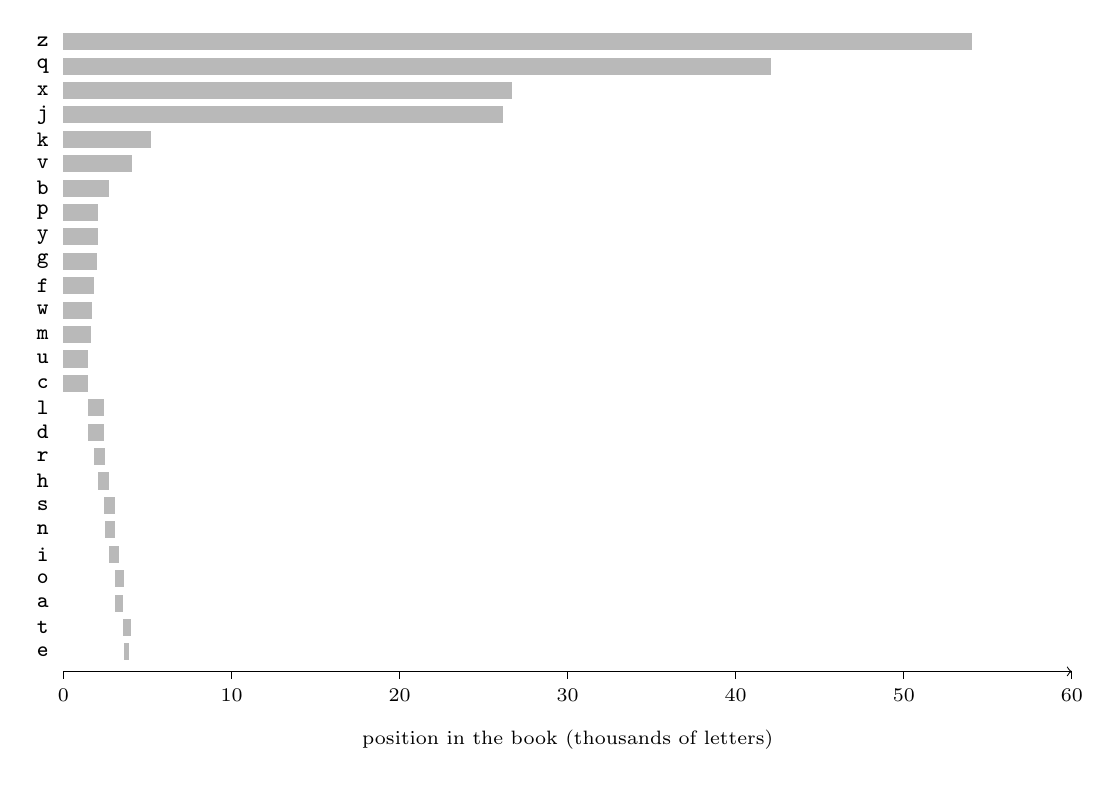
\begin{tikzpicture}[x=0.00022cm,y=0.31cm]
\fill[gray!55] (0,-0.35) rectangle (54054,0.35);
\node[anchor=east,font=\footnotesize\ttfamily] at (-300,0) {z};
\fill[gray!55] (0,-1.35) rectangle (42105,-0.65);
\node[anchor=east,font=\footnotesize\ttfamily] at (-300,-1) {q};
\fill[gray!55] (0,-2.35) rectangle (26666,-1.65);
\node[anchor=east,font=\footnotesize\ttfamily] at (-300,-2) {x};
\fill[gray!55] (0,-3.35) rectangle (26144,-2.65);
\node[anchor=east,font=\footnotesize\ttfamily] at (-300,-3) {j};
\fill[gray!55] (0,-4.35) rectangle (5181,-3.65);
\node[anchor=east,font=\footnotesize\ttfamily] at (-300,-4) {k};
\fill[gray!55] (0,-5.35) rectangle (4090,-4.65);
\node[anchor=east,font=\footnotesize\ttfamily] at (-300,-5) {v};
\fill[gray!55] (0,-6.35) rectangle (2681,-5.65);
\node[anchor=east,font=\footnotesize\ttfamily] at (-300,-6) {b};
\fill[gray!55] (0,-7.35) rectangle (2074,-6.65);
\node[anchor=east,font=\footnotesize\ttfamily] at (-300,-7) {p};
\fill[gray!55] (0,-8.35) rectangle (2026,-7.65);
\node[anchor=east,font=\footnotesize\ttfamily] at (-300,-8) {y};
\fill[gray!55] (0,-9.35) rectangle (1985,-8.65);
\node[anchor=east,font=\footnotesize\ttfamily] at (-300,-9) {g};
\fill[gray!55] (0,-10.35) rectangle (1795,-9.65);
\node[anchor=east,font=\footnotesize\ttfamily] at (-300,-10) {f};
\fill[gray!55] (0,-11.35) rectangle (1695,-10.65);
\node[anchor=east,font=\footnotesize\ttfamily] at (-300,-11) {w};
\fill[gray!55] (0,-12.35) rectangle (1662,-11.65);
\node[anchor=east,font=\footnotesize\ttfamily] at (-300,-12) {m};
\fill[gray!55] (0,-13.35) rectangle (1450,-12.65);
\node[anchor=east,font=\footnotesize\ttfamily] at (-300,-13) {u};
\fill[gray!55] (0,-14.35) rectangle (1438,-13.65);
\node[anchor=east,font=\footnotesize\ttfamily] at (-300,-14) {c};
\fill[gray!55] (1438,-15.35) rectangle (2432,-14.65);
\node[anchor=east,font=\footnotesize\ttfamily] at (-300,-15) {l};
\fill[gray!55] (1450,-16.35) rectangle (2391,-15.65);
\node[anchor=east,font=\footnotesize\ttfamily] at (-300,-16) {d};
\fill[gray!55] (1795,-17.35) rectangle (2463,-16.65);
\node[anchor=east,font=\footnotesize\ttfamily] at (-300,-17) {r};
\fill[gray!55] (2074,-18.35) rectangle (2730,-17.65);
\node[anchor=east,font=\footnotesize\ttfamily] at (-300,-18) {h};
\fill[gray!55] (2432,-19.35) rectangle (3064,-18.65);
\node[anchor=east,font=\footnotesize\ttfamily] at (-300,-19) {s};
\fill[gray!55] (2463,-20.35) rectangle (3056,-19.65);
\node[anchor=east,font=\footnotesize\ttfamily] at (-300,-20) {n};
\fill[gray!55] (2730,-21.35) rectangle (3304,-20.65);
\node[anchor=east,font=\footnotesize\ttfamily] at (-300,-21) {i};
\fill[gray!55] (3056,-22.35) rectangle (3589,-21.65);
\node[anchor=east,font=\footnotesize\ttfamily] at (-300,-22) {o};
\fill[gray!55] (3064,-23.35) rectangle (3554,-22.65);
\node[anchor=east,font=\footnotesize\ttfamily] at (-300,-23) {a};
\fill[gray!55] (3554,-24.35) rectangle (3995,-23.65);
\node[anchor=east,font=\footnotesize\ttfamily] at (-300,-24) {t};
\fill[gray!55] (3589,-25.35) rectangle (3904,-24.65);
\node[anchor=east,font=\footnotesize\ttfamily] at (-300,-25) {e};
\draw[->] (0,-25.8) -- (60000,-25.8);
\draw (0,-25.8) -- (0,-26.1) node[below,font=\scriptsize]{0};
\draw (10000,-25.8) -- (10000,-26.1) node[below,font=\scriptsize]{10};
\draw (20000,-25.8) -- (20000,-26.1) node[below,font=\scriptsize]{20};
\draw (30000,-25.8) -- (30000,-26.1) node[below,font=\scriptsize]{30};
\draw (40000,-25.8) -- (40000,-26.1) node[below,font=\scriptsize]{40};
\draw (50000,-25.8) -- (50000,-26.1) node[below,font=\scriptsize]{50};
\draw (60000,-25.8) -- (60000,-26.1) node[below,font=\scriptsize]{60};
\node[font=\scriptsize] at (30000,-28.6) {position in the book (thousands of letters)};
\end{tikzpicture}

\caption{Rare-first schedule for $\kappa=40$ and $\nu=0.25$ in the fluid model. Each bar is the interval during which a letter is in an intermediate state. Rarest letters are at the top.}\label{fig:gantt}
\end{figure}

The lesson of this analysis is not that these numbers are right, since $\kappa$ and $\nu$ are unknown and the fluid model ignores the random fluctuation of letter counts, but that the structure of the problem is set by frequency. The binding constraint is the rarest letter and not the total amount of change, so a good schedule starts the slow letters early and treats the frequent letters, which learn quickly, as a late and brief affair. It also shows that a designer who wishes to give every letter the same quality of exposure must either choose an alphabet in which the rarest letters change least, so that fewer exposures are demanded of them, or accept that rare letters will be known less well than common ones, in which case the transfer test of Section~\ref{sec:empirical} should report performance by letter frequency.

\subsection{Interference and the choice of endpoint}

Two endpoint designs give different interference structures. If the destination shapes are the existing shapes of other letters, as in a visual substitution, then the end of the book reuses the shapes of its beginning with changed meanings: the shape that meant P at the start means B at the end. The reader must overwrite an old association and not merely add a new one, and the old association is among the best practised of all. If the destination shapes are new, as in a drift from Latin to Standard Galactic, there is no overlap with beginning forms and no overwriting is needed, at the price of learning an inventory of shapes with no prior foothold. Which is easier is a hypothesis for testing and not a matter of principle, and it matters for the formal analysis in Section~\ref{sec:formal}, because it determines whether the local decodings of different parts of the book agree or conflict about the same shape.
